% Created 2016-10-14 Fri 19:28
\documentclass[smaller]{beamer}


\usetheme{metropolis}
\usepackage{fixltx2e}
\usepackage{graphicx}
\usepackage{longtable}
\usepackage{float}
\usepackage{wrapfig}
\usepackage{rotating}
\usepackage[normalem]{ulem}
\usepackage{amsmath}
\usepackage{textcomp}
\usepackage{marvosym}
\usepackage{wasysym}
\usepackage{amssymb}
\usepackage{hyperref}
\tolerance=1000
\usepackage{shellesc}
\usepackage{minted}
\usepackage{fontspec,xunicode,xltxtra}
\usepackage{tikz}
\usetikzlibrary{graphdrawing}
\usetikzlibrary{graphs}
\usegdlibrary{trees}
\setmonofont[Scale=0.7]{Menlo}
\usepackage{polyglossia}
\setmainlanguage{italian}
\newfontfamily\myunicodefallback{Menlo}
\newcommand{\keyboard}{{\color{red}\vspace{0.5cm}\fontspec[Scale=0.5]{Fira Sans SemiBold}INPUT}}
\newcommand{\screen}{{\color{blue}\vspace{0.5cm}\fontspec[Scale=0.5]{Fira Sans SemiBold}OUTPUT}\vspace{-0.2cm}}
\usepackage{fancyvrb}
\usetheme{default}
\author{Valerio Cassani, Sefano Gianelli, Riccardo Medana, Maristella Matera, Elisa Quintarelli, Letizia Tanca, Vittorio Zaccaria Vittorio Zaccaria}
\date{\today}
\title{On the Role of Context in the Design of Mobile Mashups}
\AtBeginSection[]{\begin{frame}[noframenumbering,plain]{Outline}\tableofcontents[currentsection]\end{frame}}
\hypersetup{
 pdfauthor={Valerio Cassani, Sefano Gianelli, Riccardo Medana, Maristella Matera, Elisa Quintarelli, Letizia Tanca, Vittorio Zaccaria Vittorio Zaccaria},
 pdftitle={On the Role of Context in the Design of Mobile Mashups},
 pdfkeywords={},
 pdfsubject={},
 pdfcreator={Emacs 24.5.1 (Org mode 8.3.6)}, 
 pdflang={Italian}}
\begin{document}

\maketitle
\begin{frame}{Outline}
\tableofcontents
\end{frame}


\section{Introduction}
\label{sec:orgheadline4}
\begin{frame}[label={sec:orgheadline1}]{What is this about?}
\begin{itemize}
\item \alert{An experiment}: building an app that dynamically collects, integrates and adapts data to the users’ situational needs.

\item a.k.a: \alert{CAMUS} (Context-Aware Mobile mashUpS)
\end{itemize}
\end{frame}

\begin{frame}[label={sec:orgheadline2}]{Motivation}
Bridging the best of two worlds:

\begin{itemize}
\item \alert{Context}: situational model; it allows to  
identify pertinent data sources taking into account current users’ needs

\item \alert{Mashup}: lightweight integration of heterogeneous data deployed into a mobile
app.
\end{itemize}
\end{frame}

\begin{frame}[label={sec:orgheadline3}]{Case study: tourism domain}
\begin{itemize}
\item \alert{Goal}: implement a mobile app for tourists that allows to query useful
services based on their interest/intent but still moderated by the tour operator.

\item \alert{Other requirements}: the services to be queried and the result mashup is guided by a
domain expert
\end{itemize}
\end{frame}

\section{Core functionality}
\label{sec:orgheadline10}
\begin{frame}[label={sec:orgheadline5}]{Context tree}
Design-time representation of the possible situations of use.

\begin{tikzpicture}[>=stealth,font=\tiny,
  every node/.style={circle, draw, minimum size=0.75cm},
  dimension/.style={fill=black, text=white},
      parameter/.style={thick,double,minimum size=0.25cm}
]
\graph [tree layout, grow=down, fresh nodes, level distance=0.5in, sibling distance=0.5in]
    {
        r -> {
          $d_1$ [dimension] -> { $c_{1,1}$, "..." -> $p_{1,2}$ [parameter] , "..."},
          $d_2$ [dimension] -> { "...", "..." },
          $d_3$ [dimension] -> { "...", "..." }
        }
    };
\end{tikzpicture}

where \tikz{\fill[black] (0,0) circle[radius=.5ex]} is called \alert{dimension}, 
      \tikz{\draw (0,0) circle[radius=.5ex]} is called \alert{concept\footnote{Except the root.}} and
      \tikz{\draw[thick,double] (0,0) circle[radius=.5ex]} is called \alert{parameter}.
\end{frame}

\begin{frame}[label={sec:orgheadline6}]{Example}
\begin{tikzpicture}[>=stealth,font=\tiny,
  every node/.style={circle, draw, minimum size=0.75cm},
  dimension/.style={fill=black, text=white},
      parameter/.style={thick,double,minimum size=0.25cm}
]
\graph [tree layout, grow=down, fresh nodes, level distance=0.5in, sibling distance=0.5in]
    {
        r -> {
          time [dimension] -> {morning, noon, evening, night},
          interest [dimension] -> { 
                  cinema -> { genre   [dimension] -> {
                                      thriller, comedy, "..."
                                      }, 
                              length [dimension], 
                              "..." [dimension]
                            },
                  food   -> { cuisine [dimension] -> { veggie, "..." } },
          },
          position [dimension] -> { lat -> " " [parameter], long -> " " [parameter] }
        }
    };
\end{tikzpicture}
\end{frame}


\begin{frame}[fragile,label={sec:orgheadline7}]{Context tree instance}
 \begin{itemize}
\item Given a context tree \(\mathcal{T}\), each user \(u\) will be characterized by a context tree instance 
\(t_u : \mathcal{T}\).

\item \(t_u\) will dynamically vary over time but it should be well-formed, i.e., it should have
at least an interest topic, e.g:

\item Example of \(t_u\):
\begin{verbatim}
{ 
    interest: "restaurant.veggie", 
    position: (43.1, 12.1), 
    time: "noon"
}
\end{verbatim}
\end{itemize}
\end{frame}

\begin{frame}[label={sec:orgheadline8}]{Target run time architecture}
Two tier architecture to optimize bandwidth usage.

\begin{center}
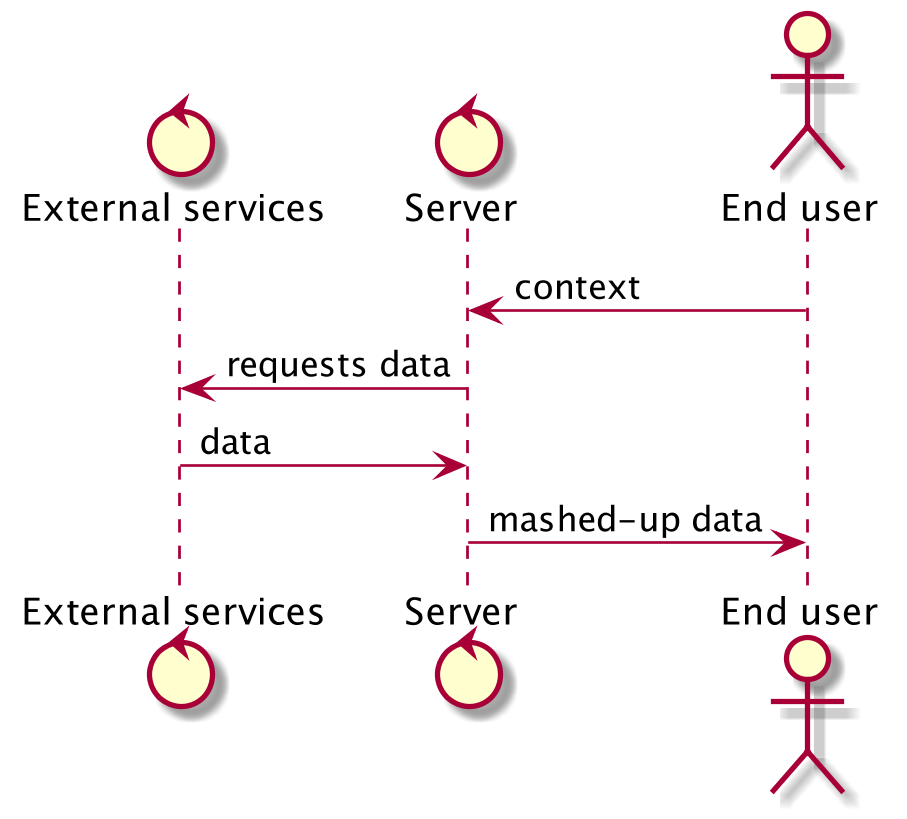
\includegraphics[height=5cm]{images/runtime.png}
\end{center}
\end{frame}

\begin{frame}[label={sec:orgheadline9}]{Principal purpose}
The \alert{principal purpose} of the system is to provide a way to map \(t_u\) to an 
ordered set of queries to services needed to satisfy the original goal:

\begin{equation}
\mathcal{C}: \mathcal{T} \rightarrow \mathcal{P}(O)
\end{equation}
\end{frame}

\section{Service selection, query and data aggregation}
\label{sec:orgheadline17}
\begin{frame}[fragile,label={sec:orgheadline11}]{Primary services}
 They are queried to \alert{fulfill} the original intent of the user (\(t_u\)). 

\begin{verbatim}
CONTEXT                       SERVICES
time = noon,                  veggieapi.com
interest = restaurant    =>   places.com?type=veg
restaurant = vegetarian       thefork?type=veggie
\end{verbatim}
\end{frame}

\begin{frame}[label={sec:orgheadline12}]{Primary service association}
Each enum's leaf \(L\) has a set \(O_L\) of operations associated with it. Each 
operation describes a request template to a service \(s\). E.g:

\begin{equation}
O_{\textrm{restaurant.vegetarian}}= \{ o_{\textrm{thefork?type=veggie}}, o_{\textrm{veggieapi}}, \ldots \}
\end{equation}

All the possible operations in the system belong to the service repository \(O\):

\begin{equation}
O = O_{L1} \cup O_{L2} \cup \ldots O_{Ln}
\end{equation}
\end{frame}

\begin{frame}[label={sec:orgheadline13}]{Primary services data mashup}
\begin{itemize}
\item Each service has its own representation of data which should be made
homogeneous before being sent to the client

\item Each response field is mapped to a \alert{term} that allows to individuate
semantically similar items.

\item Reconciliation and duplicate removal is used to remove duplicate items.
\end{itemize}
\end{frame}

\begin{frame}[fragile,label={sec:orgheadline14}]{Service selection}
 The mapping is done by categorizing leafs parents as:

\begin{itemize}
\item \alert{ranking}: leafs value in \(t_u\) will influence the order of services in the result (e.g., \texttt{position})

\item \alert{filter}: if a leaf is present in \(t_u\), it excludes services from all the siblings (e.g, if
\texttt{vegetarian : restaurant} is present, it excludes all other restaurant types).
\end{itemize}
\end{frame}

\begin{frame}[fragile,label={sec:orgheadline15}]{Support services}
 They provide the user with \alert{additional useful information}

\begin{verbatim}
CONTEXT                       SERVICES
time = evening,               maps.google.com 
interest = restaurant    =>   restaurantreviews.com
restaurant = vegetarian       uber.com
\end{verbatim}

Can be accessed either via \alert{deep-linking} or \alert{web-linking}.
\end{frame}

\begin{frame}[fragile,label={sec:orgheadline16}]{Mashup schema}
 \begin{itemize}
\item Describes how data should be visualized on the mobile device, for both \alert{list}
  and \alert{detail} views.

\item It is downloaded at login and guides the view creation once results are
received.

\item Example:

\begin{verbatim}
CONTEXT                       MASHUP (DETAILS)
...                           name: text
interest = restaurant    =>   address: text
...                           (long, lat): map
\end{verbatim}
\end{itemize}
\end{frame}

\section{Client and Server implementation}
\label{sec:orgheadline24}
\begin{frame}[label={sec:orgheadline18}]{Requirements}
\begin{itemize}
\item \alert{Minimize bandwidth usage}: ask only for what you need

\item \alert{Custom response types}: different context may need different types of data

\item \alert{Native app feeling}: native app still better performance-wise and battery-wise.
\end{itemize}
\end{frame}

\begin{frame}[label={sec:orgheadline19}]{}

\includegraphics{./images/jsatt.jpg} 
\end{frame}

\begin{frame}[label={sec:orgheadline20}]{GraphQL}
\begin{itemize}
\item Data-fetching API that returns JSON
\item Query defines a data shape
\begin{itemize}
\item easy to add field leaving existing clients unaffected
\item optimal bandwidth usage
\end{itemize}
\item It can be hierarchical: it naturally follows relationships between objects
\end{itemize}
\end{frame}

\begin{frame}[fragile,label={sec:orgheadline21}]{GraphQL example}
 \begin{minted}[obeytabs=true,baselinestretch=0.95]{js}
executeQuery(id: "56975a1bd5704e0d0d815869", t_u) { shape }
\end{minted}

where \texttt{t\_u} is a json-like representation of \(t_u\), while 
\alert{shape} describes the data set needed:


\begin{minted}[obeytabs=true,baselinestretch=0.95]{js}
primaryResults {
    edges {
        node {
            title,
            address,
            telephone,
            website
        }
    }
}
\end{minted}
\end{frame}

\begin{frame}[label={sec:orgheadline22}]{React and React Native}
\begin{itemize}
\item React abstracts away the DOM, giving a simpler programming model and better performance

\item It implements one-way reactive data flow which reduces boilerplate and is easier to reason about than traditional data binding
\end{itemize}
\end{frame}

\begin{frame}[fragile,label={sec:orgheadline23}]{React Native / Example}
 \begin{minted}[obeytabs=true,baselinestretch=0.95]{js}
class App extends Component {
  render() {
    return (
      <TabBarIOS>
        <TabBarIOS.Item title="React Native" selected={true}>
          <NavigatorIOS initialRoute={{ title: 'React Native' }} />
        </TabBarIOS.Item>
      </TabBarIOS>
    );
  }
}
\end{minted}
\end{frame}

\section{Live Demo}
\label{sec:orgheadline25}

\section{Performance evaluation}
\label{sec:orgheadline28}
\begin{frame}[label={sec:orgheadline26}]{Time breakout}
\begin{center}
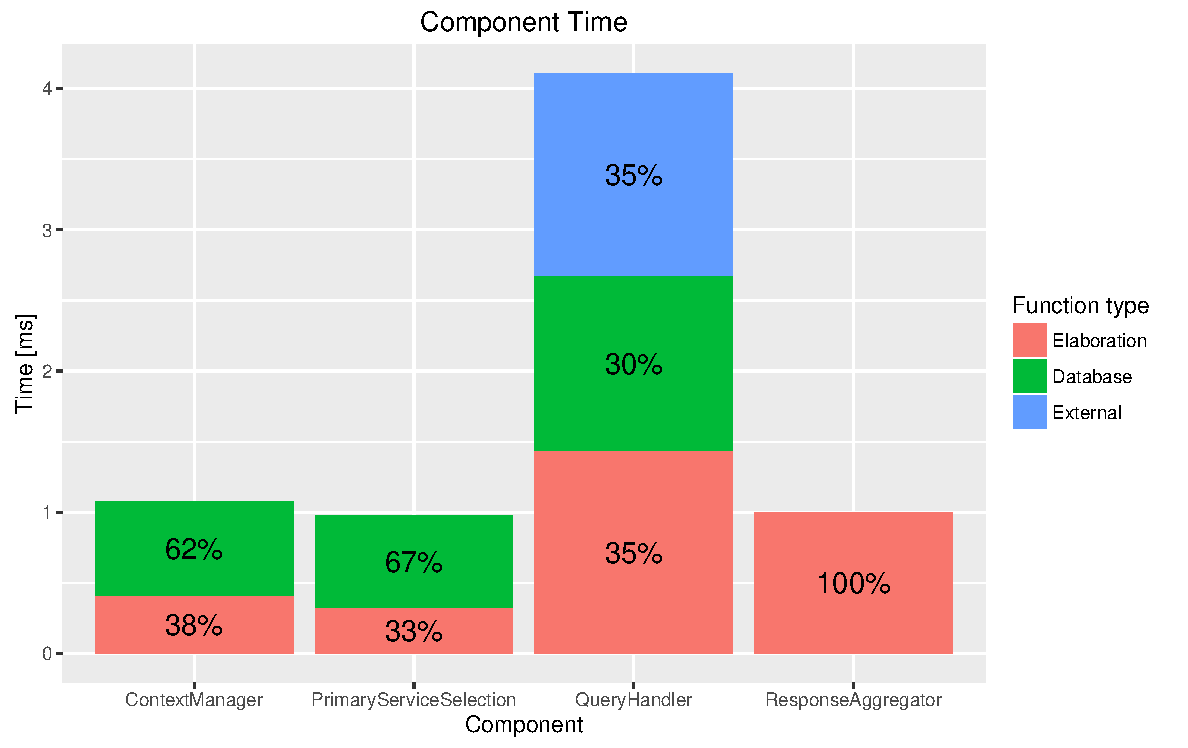
\includegraphics{./images/component_time.pdf}
\end{center}
\end{frame}

\begin{frame}[label={sec:orgheadline27}]{Scaling}
\begin{center}
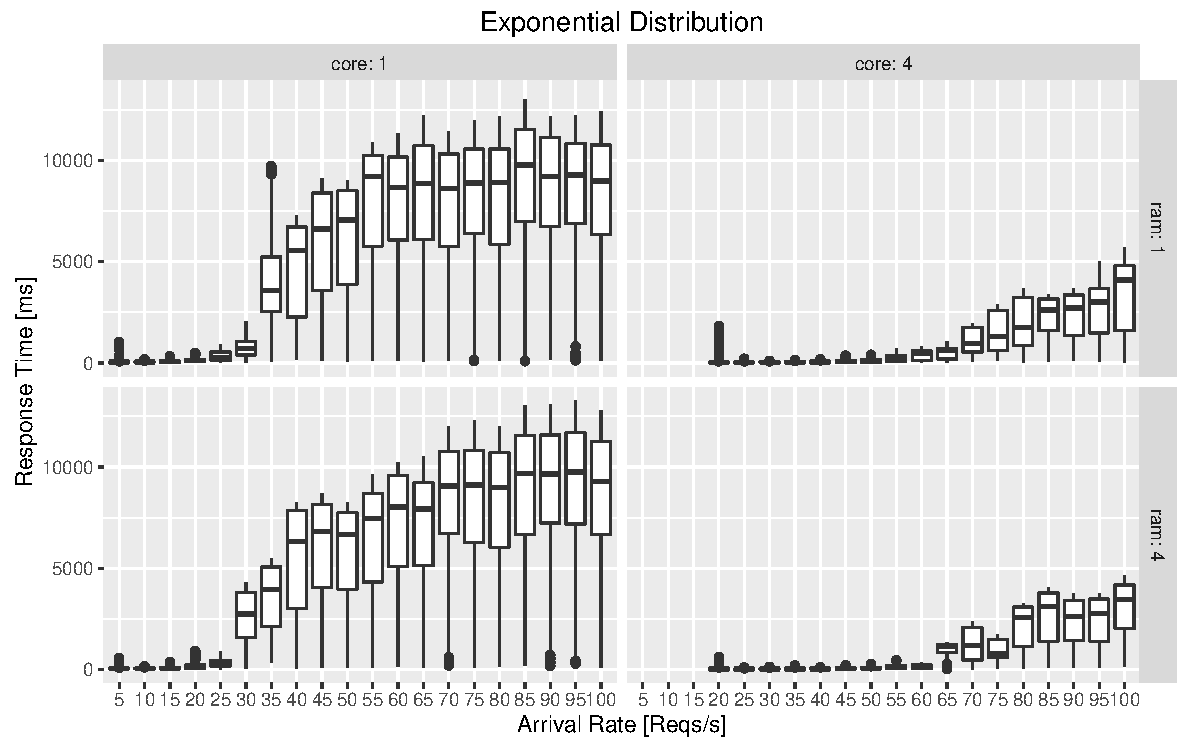
\includegraphics{./images/exponential_analysis.pdf}
\end{center}
\end{frame}

\section{Conclusions}
\label{sec:orgheadline30}
\begin{frame}[label={sec:orgheadline29}]{What still needs to be done}
\begin{itemize}
\item Better formalization of the query represented by the context

\item Extension to services with a SOAP interface
\end{itemize}
\end{frame}


\section{Detailed description}
\label{sec:orgheadline32}
\begin{frame}[label={sec:orgheadline31}]{Administrator and domain expert roles}
\begin{center}
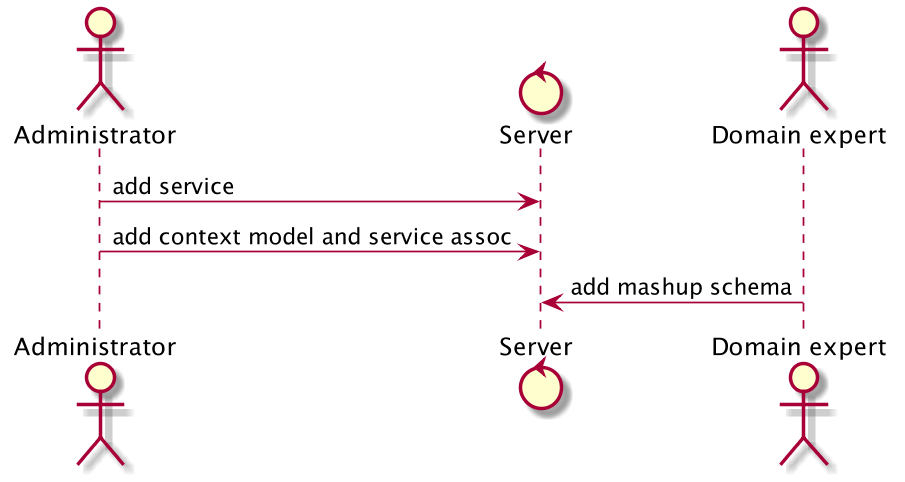
\includegraphics{images/designtime.png}
\end{center}
\end{frame}
\end{document}